\documentclass{article}
\usepackage{tikz}
\usetikzlibrary{arrows}
\usetikzlibrary[topaths]


\newcount\mycount



\begin{document}

\begin{abstract}
 
Boolean networks have been successfully applied to model gene regulatory networks. Inspired by \cite{Goudarzi} we started to couple boolean with metabolic 
networks to observe their evolution. To do that, we numerically implemented a fixed size population of organisms which divide upon accumulating biomass. 
This is achieved depending on their correct switching of reactions and the consequent production of a target molecule, similar to a percolation in the 
metabolism of that organism. A biomass penalty proportional to the number of enzymes being produced is applied to them, in order to avoid the trivial 
solution (all reactions on).  Each organism has its own boolean network and whenever it divides it produces an exact copy and a mutant one. The food 
molecules in the metabolic network are also present as ingoing nodes in the boolean network, acting thus as sensors of a varying environment. 
Some boolean nodes represent enzymes in the metabolism and turns the corresponding reaction on. This effectively couples both networks of each individual. 
The topology of the metabolic network is shared by all individuals of a population, and different topologies are being proposed as different tasks for the 
populations to solve.

\end{abstract}

The main idea consists of observing how the organisms in a population evolve their gene regulatory structure according to the availability of nutrients. 
To achieve that, we constructed organisms that couple the metabolic network with their boolean network. 

The boolean network is composed by $N$ genes that may have only two states, $\sigma_i \in \{0,1\}$ and a certain interaction topology. 
Every gene may potentially repress or enhance other genes, and we define a weight $w_{ij} \in \{-1,0,1\}$ for the efect that gene $i$ has on gene $j$. This is 
not necessarily symmetric. The metabolic network is a bipartite directed network composed by reaction nodes and chemical species nodes. 


We couple these two types of networks in the intuitive way: whenever a gene $i$ is switched on, if there is a corresponding chemical reaction in which it 
works as an enzyme it will promote that reaction in case the educts are all present within the cell (of that organism); and to sense the presence of some 
metabolites we can also send the signal from the metabolic network to the boolean network. These nodes in the boolean network that work as sensors are not 
genes. The Figure~\ref{general} shows a general scheme


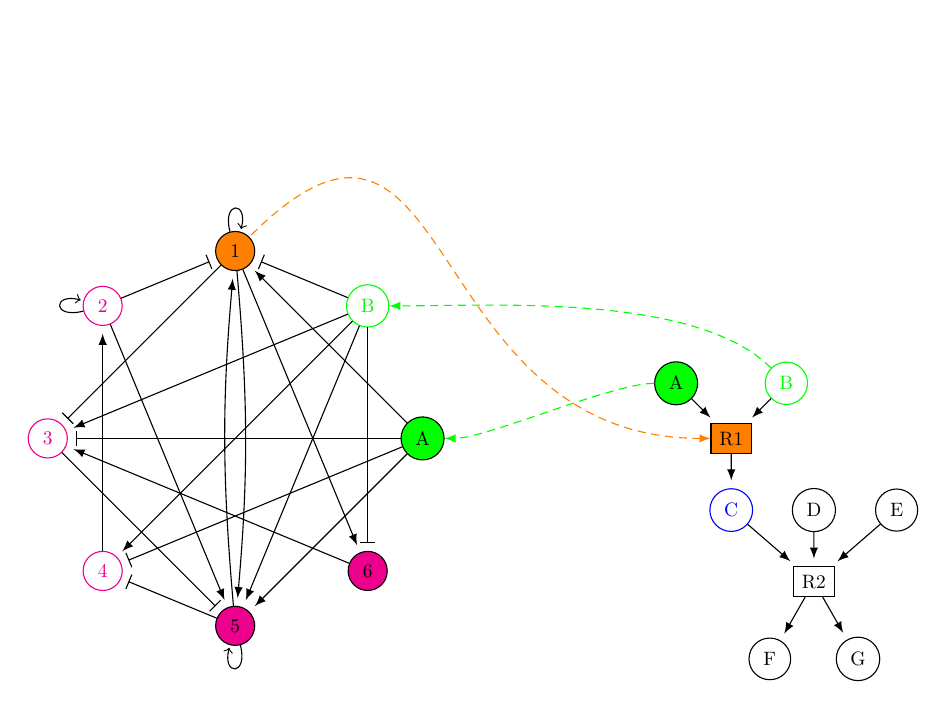
\begin{tikzpicture}[scale=0.7,transform shape]
  
  \node[draw,circle,inner sep=0.15cm,fill=green] (A1) at (0:3.4cm) {A};
  \node[draw,circle,inner sep=0.15cm,green] (B1) at (45:3.4cm) {B};
  \node[draw,circle,inner sep=0.15cm,fill=orange] (1) at (90:3.4cm) {1};
  \node[draw,circle,inner sep=0.15cm, magenta] (2) at (135:3.4cm) {2};
  \node[draw,circle,inner sep=0.15cm, magenta] (3) at (180:3.4cm) {3};
  \node[draw,circle,inner sep=0.15cm, magenta] (4) at (225:3.4cm) {4};
  \node[draw,circle,inner sep=0.15cm, fill=magenta] (5) at (270:3.4cm) {5};
  \node[draw,circle,inner sep=0.15cm, fill=magenta] (6) at (315:3.4cm) {6};

  \node[draw,circle,inner sep=0.15cm,fill=green] (A2) at (8cm,1cm) {A};
  \node[draw,circle,inner sep=0.15cm,green] (B2) at (10cm,1cm) {B};
  \node[draw,shape=rectangle,inner sep=0.15cm,fill=orange] (R) at (9cm,0cm) {R1};
  \node[draw,circle,inner sep=0.15cm,blue] (C) at (9cm,-1.3cm) {C};
  \node[draw,circle,inner sep=0.15cm] (D) at (10.5cm,-1.3cm) {D};
  \node[draw,circle,inner sep=0.15cm] (E) at (12cm,-1.3cm) {E};
  \node[draw,shape=rectangle,inner sep=0.15cm] (R2) at (10.5cm,-2.6cm) {R2};
  \node[draw,circle,inner sep=0.15cm] (F) at (9.7cm,-4cm) {F};
  \node[draw,circle,inner sep=0.15cm] (G) at (11.3cm,-4cm) {G};

  \draw[shorten >=0.1cm,-latex] (A2) edge (R);
  \draw[shorten >=0.1cm,-latex] (B2) edge (R);
  \draw[shorten >=0.1cm,-latex] (R) edge (C);
  \draw[shorten >=0.1cm,-latex] (C) edge (R2);
  \draw[shorten >=0.1cm,-latex] (D) edge (R2);
  \draw[shorten >=0.1cm,-latex] (E) edge (R2);
  \draw[shorten >=0.1cm,-latex] (R2) edge (F);
  \draw[shorten >=0.1cm,-latex] (R2) edge (G);



  \path (A2) edge[-latex,green, out=180, in=0,densely dashed,looseness=0.5] (A1)
        (B2) edge[-latex,green, out=135, in=0,densely dashed,looseness=0.7] (B1)
        (R) edge[latex-,orange, out=180, in=45,densely dashed,looseness=1.5] (1);

  \draw[shorten >=0.1cm,-latex] (A1) edge (1);
  \draw[shorten >=0.1cm,-|] (A1) edge (3);
  \draw[shorten >=0.1cm,-|] (A1) edge (4);
  \draw[shorten >=0.1cm,-latex] (A1) edge (5);
  \draw[shorten >=0.1cm,-|] (B1) edge (1);
  \draw[shorten >=0.1cm,-latex] (B1) edge (3);
  \draw[shorten >=0.1cm,-latex] (B1) edge (4);
  \draw[shorten >=0.1cm,-latex] (B1) edge (5);
  \draw[shorten >=0.1cm,-|] (B1) edge (6);
  \draw[shorten >=0.1cm,-latex] (1) edge [loop above] (1);
  \draw[shorten >=0.1cm,-|] (1) edge (3);
  \draw[shorten >=0.1cm,-latex] (1) edge [bend left=5] (5);
  \draw[shorten >=0.1cm,-latex] (1) edge (6);
  \draw[shorten >=0.1cm,-|] (2) edge (1);
  \draw[shorten >=0.1cm,-latex] (2) edge [loop left] (2);
  \draw[shorten >=0.1cm,-latex] (2) edge (5);
  \draw[shorten >=0.1cm,-|] (3) edge (5);
  \draw[shorten >=0.1cm,-latex] (4) edge (2);
  \draw[shorten >=0.1cm,-latex] (5) edge [bend left=5] (1);
  \draw[shorten >=0.1cm,-|] (5) edge (4);
  \draw[shorten >=0.1cm,-latex] (5) edge [loop below] (5);
  \draw[shorten >=0.1cm,-latex] (6) edge (3);

\label{general}
\end{tikzpicture}


\vspace{1cm}

\begin{equation}
\sigma_i^{t+1} = \Theta(\sum_{j}\omega_{ji}\sigma_j^t - \theta_i)
\end{equation}


where

\[
  \Theta(x) = \left\{ 
  \begin{array}{l l}
    1 & \quad \textrm{if $x > 0$} \\
    0 & \quad \textrm{otherwise}
  \end{array} \right.
\]


\vspace{1cm}

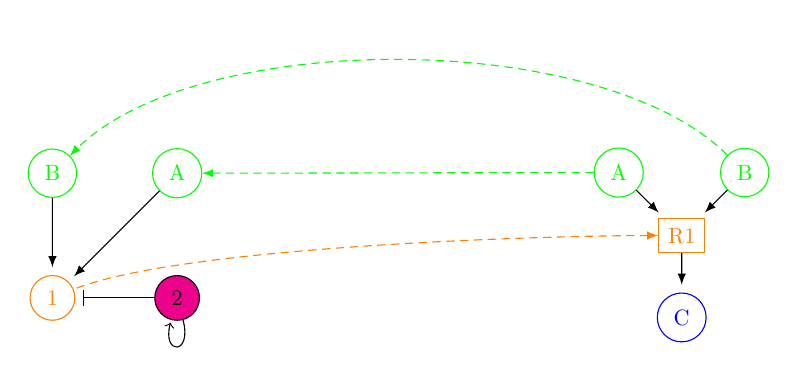
\begin{tikzpicture}[scale=0.8,transform shape]
  
  \node[draw,circle,inner sep=0.15cm,green] (A1) at (45:1.4cm) {A};
  \node[draw,circle,inner sep=0.15cm,green] (B1) at (135:1.4cm) {B};
  \node[draw,circle,inner sep=0.15cm,orange] (1) at (225:1.4cm) {1};
  \node[draw,circle,inner sep=0.15cm, fill=magenta] (2) at (315:1.4cm) {2};

  \node[draw,circle,inner sep=0.15cm,green] (A2) at (8cm,1cm) {A};
  \node[draw,circle,inner sep=0.15cm,green] (B2) at (10cm,1cm) {B};
  \node[draw,shape=rectangle,inner sep=0.15cm,orange] (R) at (9cm,0cm) {R1};
  \node[draw,circle,inner sep=0.15cm,blue] (C) at (9cm,-1.3cm) {C};

  \draw[shorten >=0.1cm,-latex] (A2) edge (R);
  \draw[shorten >=0.1cm,-latex] (B2) edge (R);
  \draw[shorten >=0.1cm,-latex] (R) edge (C);


  \path (A2) edge[-latex,green, out=180, in=0,densely dashed,looseness=0.5] (A1)
        (B2) edge[-latex,green, out=135, in=45,densely dashed,looseness=0.7] (B1)
        (R) edge[latex-,orange, out=180, in=22,densely dashed,looseness=0.5] (1);

  \draw[shorten >=0.1cm,-latex] (A1) edge (1);
  \draw[shorten >=0.1cm,-latex] (B1) edge (1);
  \draw[shorten >=0.1cm,-|] (2) edge (1);
  \draw[shorten >=0.1cm,-latex] (2) edge [loop below] (2);

\end{tikzpicture}

\vspace{2cm}

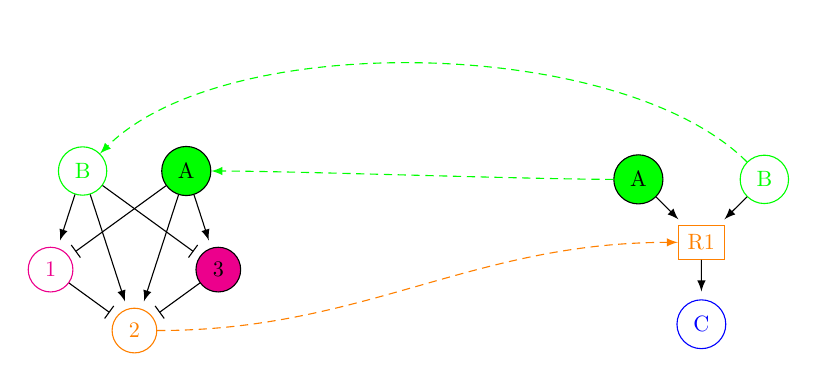
\begin{tikzpicture}[scale=0.8,transform shape]
  
  \node[draw,circle,inner sep=0.15cm,fill=green] (A1) at (54:1.4cm) {A};
  \node[draw,circle,inner sep=0.15cm,green] (B1) at (126:1.4cm) {B};
  \node[draw,circle,inner sep=0.15cm,magenta] (1) at (198:1.4cm) {1};
  \node[draw,circle,inner sep=0.15cm, orange] (2) at (270:1.4cm) {2};
  \node[draw,circle,inner sep=0.15cm, fill=magenta] (3) at (342:1.4cm) {3};

  \node[draw,circle,inner sep=0.15cm,fill=green] (A2) at (8cm,1cm) {A};
  \node[draw,circle,inner sep=0.15cm,green] (B2) at (10cm,1cm) {B};
  \node[draw,shape=rectangle,inner sep=0.15cm,orange] (R) at (9cm,0cm) {R1};
  \node[draw,circle,inner sep=0.15cm,blue] (C) at (9cm,-1.3cm) {C};

  \draw[shorten >=0.1cm,-latex] (A2) edge (R);
  \draw[shorten >=0.1cm,-latex] (B2) edge (R);
  \draw[shorten >=0.1cm,-latex] (R) edge (C);


  \path (A2) edge[-latex,green, out=180, in=0,densely dashed,looseness=0.5] (A1)
        (B2) edge[-latex,green, out=135, in=45,densely dashed,looseness=0.7] (B1)
        (R) edge[latex-,orange, out=180, in=0,densely dashed,looseness=1.0] (2);

  \draw[shorten >=0.1cm,-latex] (A1) edge (2);
  \draw[shorten >=0.1cm,-latex] (B1) edge (2);
  \draw[shorten >=0.1cm,-latex] (B1) edge (1);
  \draw[shorten >=0.1cm,-|] (B1) edge (3);
  \draw[shorten >=0.1cm,-|] (A1) edge (1);
  \draw[shorten >=0.1cm,-latex] (A1) edge (3);
  \draw[shorten >=0.1cm,-|] (1) edge (2);
  \draw[shorten >=0.1cm,-|] (3) edge (2);


\end{tikzpicture}

\vspace{2cm}


\begin{tikzpicture}[scale=0.8,transform shape]
  
  \node[draw,circle,inner sep=0.15cm,green] (A1) at (30:1.4cm) {A};
  \node[draw,circle,inner sep=0.15cm,green] (B1) at (150:1.4cm) {B};
  \node[draw,circle,inner sep=0.15cm,orange] (1) at (270:1.4cm) {1};

  \node[draw,circle,inner sep=0.15cm,green] (A2) at (8cm,1cm) {A};
  \node[draw,circle,inner sep=0.15cm,green] (B2) at (10cm,1cm) {B};
  \node[draw,shape=rectangle,inner sep=0.15cm,orange] (R) at (9cm,0cm) {R1};
  \node[draw,circle,inner sep=0.15cm,blue] (C) at (9cm,-1.3cm) {C};

  \draw[shorten >=0.1cm,-latex] (A2) edge (R);
  \draw[shorten >=0.1cm,-latex] (B2) edge (R);
  \draw[shorten >=0.1cm,-latex] (R) edge (C);


  \path (A2) edge[-latex,green, out=180, in=0,densely dashed,looseness=0.5] (A1)
        (B2) edge[-latex,green, out=135, in=45,densely dashed,looseness=0.7] (B1)
        (R) edge[latex-,orange, out=180, in=22,densely dashed,looseness=0.5] (1);

  \draw[shorten >=0.1cm,-latex] (A1) edge (1);
  \draw[shorten >=0.1cm,-|] (B1) edge (1);
  \draw[shorten >=0.1cm,-latex] (1) edge [loop below] (1);


\end{tikzpicture}


\vspace{2cm}

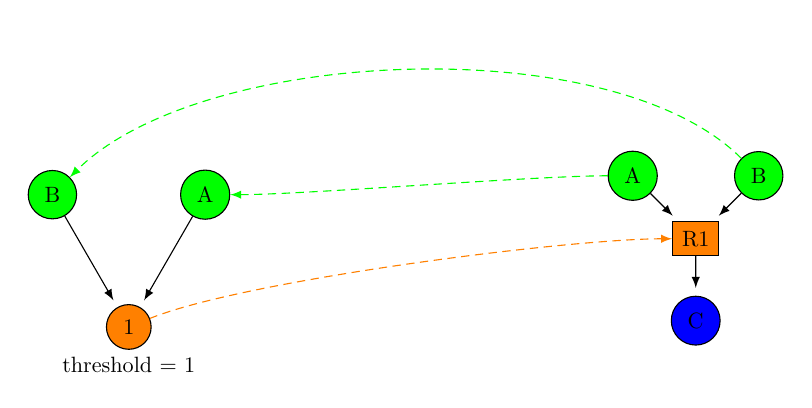
\begin{tikzpicture}[scale=0.8,transform shape]
  
  \node[draw,circle,inner sep=0.15cm,fill=green] (A1) at (30:1.4cm) {A};
  \node[draw,circle,inner sep=0.15cm,fill=green] (B1) at (150:1.4cm) {B};
  \node[draw,circle,inner sep=0.15cm,fill=orange] (1) at (270:1.4cm) {1};
  \node (label) at (270:2cm) {threshold = 1};

  \node[draw,circle,inner sep=0.15cm,fill=green] (A2) at (8cm,1cm) {A};
  \node[draw,circle,inner sep=0.15cm,fill=green] (B2) at (10cm,1cm) {B};
  \node[draw,shape=rectangle,inner sep=0.15cm,fill=orange] (R) at (9cm,0cm) {R1};
  \node[draw,circle,inner sep=0.15cm,fill=blue] (C) at (9cm,-1.3cm) {C};

  \draw[shorten >=0.1cm,-latex] (A2) edge (R);
  \draw[shorten >=0.1cm,-latex] (B2) edge (R);
  \draw[shorten >=0.1cm,-latex] (R) edge (C);


  \path (A2) edge[-latex,green, out=180, in=0,densely dashed,looseness=0.5] (A1)
        (B2) edge[-latex,green, out=135, in=45,densely dashed,looseness=0.7] (B1)
        (R) edge[latex-,orange, out=180, in=22,densely dashed,looseness=0.5] (1);

  \draw[shorten >=0.1cm,-latex] (A1) edge (1);
  \draw[shorten >=0.1cm,-latex] (B1) edge (1);


\end{tikzpicture}

\vspace{2cm}


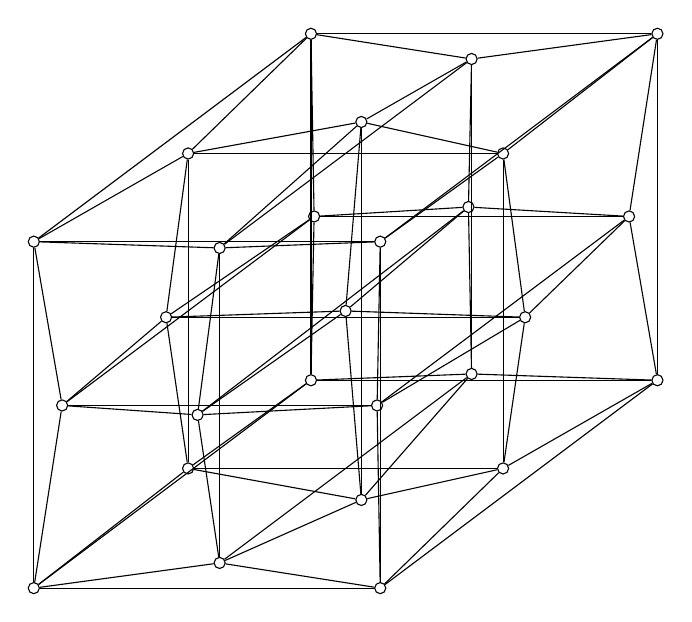
\begin{tikzpicture}[scale=0.4]

\node[draw,circle,inner sep=0.05cm] (0) at (-9.9,-8.8) {};   
\node[draw,circle,inner sep=0.05cm] (1) at (-4,-8) {};%
\node[draw,circle,inner sep=0.05cm] (2) at (1.1,-8.8) {};
\node[draw,circle,inner sep=0.05cm] (3) at (-5,-5) {};%
\node[draw,circle,inner sep=0.05cm] (4) at (0.5,-6) {};%%
\node[draw,circle,inner sep=0.05cm] (5) at (5,-5) {};%
\node[draw,circle,inner sep=0.05cm] (6) at (-1.1,-2.2) {};
\node[draw,circle,inner sep=0.05cm] (7) at (4,-2) {};%
\node[draw,circle,inner sep=0.05cm] (8) at (9.9,-2.2) {};
\node[draw,circle,inner sep=0.05cm] (9) at (-9,-3) {};%
\node[draw,circle,inner sep=0.05cm] (10) at (-4.7,-3.3) {};%%
\node[draw,circle,inner sep=0.05cm] (11) at (1,-3) {};%
\node[draw,circle,inner sep=0.05cm] (12) at (-5.7,-0.2) {};%%
\node[draw,circle,inner sep=0.05cm] (13) at (0,0) {};%                                       
\node[draw,circle,inner sep=0.05cm] (14) at (5.7,-0.2) {};%%                                       
\node[draw,circle,inner sep=0.05cm] (15) at (-1,3) {};%                                    
\node[draw,circle,inner sep=0.05cm] (16) at (3.9,3.3) {};%%
\node[draw,circle,inner sep=0.05cm] (17) at (9,3) {};%
\node[draw,circle,inner sep=0.05cm] (18) at (-9.9,2.2) {};
\node[draw,circle,inner sep=0.05cm] (19) at (-4,2) {};%
\node[draw,circle,inner sep=0.05cm] (20) at (1.1,2.2) {};
\node[draw,circle,inner sep=0.05cm] (21) at (-5,5) {};%
\node[draw,circle,inner sep=0.05cm] (22) at (0.5,6) {};%%
\node[draw,circle,inner sep=0.05cm] (23) at (5,5) {};%
\node[draw,circle,inner sep=0.05cm] (24) at (-1.1,8.8) {};
\node[draw,circle,inner sep=0.05cm] (25) at (4,8) {};%
\node[draw,circle,inner sep=0.05cm] (26) at (9.9,8.8) {};

\draw (0) edge (1);
\draw (1) edge (2);
\draw (2) edge (0);
\draw (3) edge (4);
\draw (4) edge (5);
\draw (5) edge (3);
\draw (6) edge (7);
\draw (7) edge (8);
\draw (8) edge (6);
\draw (9) edge (10);
\draw (10) edge (11);
\draw (11) edge (9);
\draw (12) edge (13);
\draw (13) edge (14);
\draw (14) edge (12);
\draw (15) edge (16);
\draw (16) edge (17);
\draw (17) edge (15);
\draw (18) edge (19);
\draw (19) edge (20);
\draw (20) edge (18);
\draw (21) edge (22);
\draw (22) edge (23);
\draw (23) edge (21);
\draw (24) edge (25);
\draw (25) edge (26);
\draw (26) edge (24);

\draw (0) edge (3);
\draw (3) edge (6);
\draw (6) edge (0);
\draw (1) edge (4);
\draw (4) edge (7);
\draw (7) edge (1);
\draw (2) edge (5);
\draw (5) edge (8);
\draw (8) edge (2);
\draw (9) edge (12);
\draw (12) edge (15);
\draw (15) edge (9);
\draw (10) edge (13);
\draw (13) edge (16);
\draw (16) edge (10);
\draw (11) edge (14);
\draw (14) edge (17);
\draw (17) edge (11);
\draw (18) edge (21);
\draw (21) edge (24);
\draw (24) edge (18);
\draw (19) edge (22);
\draw (22) edge (25);
\draw (25) edge (19);
\draw (20) edge (23);
\draw (23) edge (26);
\draw (26) edge (20);

\draw (0) edge (9);
\draw (9) edge (18);
\draw (18) edge (0);
\draw (1) edge (10);
\draw (10) edge (19);
\draw (19) edge (1);
\draw (2) edge (11);
\draw (11) edge (20);
\draw (20) edge (2);
\draw (3) edge (12);
\draw (12) edge (21);
\draw (21) edge (3);
\draw (4) edge (13);
\draw (13) edge (22);
\draw (22) edge (4);
\draw (5) edge (14);
\draw (14) edge (23);
\draw (23) edge (5);
\draw (6) edge (15);
\draw (15) edge (24);
\draw (24) edge (6);
\draw (7) edge (16);
\draw (16) edge (25);
\draw (25) edge (7);
\draw (8) edge (17);
\draw (17) edge (26);
\draw (26) edge (8);




\end{tikzpicture}



\end{document}

